\chapter{MARCO TEÓRICO} 
	
	\vspace{0pt}
	
	\section{LOGÍSTICA DEL TRANSPORTE DE PASAJEROS}
	\subsection{Logística}
		``Logística es planificar, operar, controlar y detectar oportunidades de mejora del proceso de flujo de materiales (insumos, productos), servicios, información y dinero.  Es la función que normalmente opera como nexo entre las fuentes de aprovisionamiento y suministro y el cliente final o la distribución.  Su objetivo es satisfacer permanentemente la demanda en cuanto a cantidad, oportunidad y calidad al menor costo posible para la empresa.''\parencite{carro2013logistica}
	\subsection{Transporte}
		Según \textcite{koch2001transporte}: ``El concepto de “transporte” hace referencia al traslado de personas y mercancías de un lugar a otro por diversas razones en el menor tiempo posible. En el caso de las personas, destacan los motivos laborales, de estudio o de satisfacción de otras necesidades como el ocio, el acceso a servicios de salud, entre otros; en
		el caso de las mercancías, la necesidad de producción de bienes industriales y de consumo y la posterior comercialización de estos hacen del proceso de transporte un elemento central.'' Por su parte en la \textcite{ley2011transporte}: ``Se denomina transporte al traslado de un lugar a otro de personas y carga.''
		
		
		El transporte es un componente de la logística, que se refiere al conjunto de recursos y estrategias utilizados para organizar un servicio o administrar una empresa. En el ámbito comercial, la logística se relaciona con el envío de productos al lugar adecuado, en el momento correcto y bajo las condiciones necesarias. Por lo tanto, el transporte de mercancías es una parte integral de la logística. El propósito de una empresa es asegurar que la distribución y venta de sus productos se realice de manera eficiente y al menor costo posible. En este contexto, el transporte abarca tanto los vehículos como las infraestructuras asociadas, como camiones, barcos, trenes de carga, carreteras y puertos.
		
		También existen dos tipos de transporte, el público y el privado.
		
		Se habla de transporte público, para hacer referencia a los autobuses, trenes y otras unidades móviles que sirven para la movilización de los ciudadanos de una comunidad y que está solventado y manejado por el Estado vigente. Cabe señalar que en algunos casos, dichos coches pertenecen a empresas privadas que tienen algún tipo de acuerdo con el gobierno y han asumido la responsabilidad de brindar un servicio determinado a la comunidad. Resulta importante señalar que esta clase de transporte no tiene como propósito la generación de ganancias, sino que debe cumplir con un fin social y ser útil para la comunidad. Por ejemplo: “Los transportes públicos están colapsados y requieren de mayores inversiones para
		poder satisfacer las necesidades de la población”.
		
		El transporte privado, en cambio, es el que pertenece a individuos o empresas particulares. En este caso los responsables de la manutención de dichos vehículos son sus dueños, al igual que serán quienes respondan por ellos en caso de
		accidente.
	\subsection{Pasajero}
		En la \textcite{ley_municipal2012transporte} en su artículo 59 se define a los usuarios o pasajeros como ``Las personas naturales o jurídicas que utilizan un vehículo del servicio público o privado de transporte, para trasladarse de un origen a un destino a cambio de una tarifa establecida o remuneración convenida, son considerados usuarios o pasajeros en el marco de la presente Ley Municipal.''
	
	\subsection{Sistema de transporte}
		De acuerdo con \textcite{garcía2016gestión}: ``Un sistema de transporte desde la perspectiva informática es una red interconectada de componentes físicos y digitales que utiliza tecnologías avanzadas de información y comunicación para optimizar el flujo de personas y mercancías. Incluye sistemas de gestión de tráfico, planificación de rutas en tiempo real, control de flotas y plataformas de información al usuario, todos ellos integrados mediante software especializado y bases de datos.''
	% \subsection{Funcionalidad del transporte}
	\section{RESERVA Y VENTA DE PASAJES}
	\subsection{Proceso de reserva y venta de pasajes}
		El proceso de reserva y venta de pasajes es un componente fundamental en la operación de cualquier empresa de transporte de pasajeros. Según \textcite{aparicio2013gestion}, este proceso implica una serie de pasos secuenciales que permiten al cliente asegurar su lugar en un viaje específico. Tradicionalmente, las empresas de transporte han utilizado diversos canales para la reserva y venta, incluyendo puntos de venta físicos, call centers, y más recientemente, plataformas en línea.	
	\subsection{Emisión y gestion de boletos}
		La emisión y gestión de boletos es un proceso crítico que ha evolucionado significativamente con la tecnología. \textcite{agenjo2008transporte} describen dos tipos principales de boletos en el transporte moderno: los electrónicos (e-tickets) y los impresos tradicionales. Independientemente del formato, los boletos deben contener información esencial como datos del pasajero, detalles del viaje, asiento asignado y un método de validación.
		
		El proceso de emisión, según \textcite{garcía2016gestión}, debe ser ágil y estar vinculado directamente con la confirmación del pago. La gestión eficiente de boletos implica un sistema robusto de validación, ya sea en terminales o a bordo de los vehículos, así como la capacidad de reimpresión en caso de pérdida. Además, como señala \textcite{robuste2005logistica}, el seguimiento y registro de los boletos emitidos es importante para el control operativo y financiero de la empresa de transporte.
	\subsection{Cambios y cancelaciones}
		La gestión de cambios y cancelaciones es un aspecto delicado que requiere un equilibrio entre la flexibilidad para los clientes y la protección de los intereses de la empresa. Según \textcite{tejero2015transporte}, las políticas de cambios y cancelaciones deben ser claras, especificando plazos permitidos y cargos aplicables.
		
		El proceso de solicitud de cambios, como describe \textcite{ramírez2015logística}, implica la verificación de disponibilidad para nuevas fechas y el cálculo de diferencias tarifarias. En cuanto a las cancelaciones, el sistema debe determinar el monto del reembolso según la política establecida. La gestión de reembolsos, de acuerdo con \textcite{garcía2016gestión}, debe ser eficiente y transparente, ofreciendo múltiples métodos según las preferencias del cliente.
		
		Un aspecto importante señalado por \textcite{rivera2002ESTUDIODL} es la reasignación de asientos liberados, lo que permite optimizar la ocupación de los vehículos. Además, el registro detallado de cambios y cancelaciones proporciona datos valiosos para el análisis de patrones de comportamiento de los clientes y la mejora continua de los servicios.
		
		En conjunto, estos procesos de reserva, emisión de boletos y gestión de cambios y cancelaciones forman la columna vertebral de la operación de venta de pasajes en una empresa de transporte. Su eficiente implementación y gestión son cruciales para la satisfacción del cliente y el éxito operativo de la empresa.
	\section{LOGÍSTICA DE ENVÍO DE ENCOMIENDAS}
	\subsection{Encomienda}
		La encomienda es el objeto o paquete que se transporta de un punto a otro a través de un servicio de mensajería o transporte. Según \textcite{stock2000strategic}, ``una encomienda representa una unidad logística que debe ser gestionada y tratada como tal, garantizando su integridad desde el origen hasta el destino final''. En el contexto del transporte de encomiendas, es fundamental contar con un sistema que permita la correcta identificación, seguimiento y gestión de cada paquete.
		
		\textcite{garcía2016gestión} destaca que el concepto de encomienda ha evolucionado con el tiempo, especialmente con el auge del comercio electrónico. Actualmente, las empresas de transporte deben estar preparadas para manejar una amplia gama de artículos, desde documentos hasta productos perecederos, cada uno con sus propios requisitos de manipulación y transporte. Esta diversidad exige sistemas flexibles y adaptables que puedan responder a las necesidades cambiantes de los clientes y del mercado.
	\subsection{Proceso de recepción}
		El proceso de recepción es la primera etapa en la gestión de encomiendas, donde se verifica la información proporcionada por el remitente, se inspecciona el paquete y se registran los detalles necesarios para su envío. De acuerdo con \textcite{garcía2016gestión}, este proceso implica la verificación inicial del paquete, el registro de información relevante y la asignación de un identificador único. \textcite{escudero2019logistica} enfatiza la importancia de este paso para garantizar la trazabilidad y el manejo adecuado de la encomienda durante todo su trayecto.
		
		Con el avance de las tecnologías, muchas empresas han implementado sistemas que automatizan el proceso de recepción, permitiendo la digitalización de la información desde el inicio del proceso logístico. Esto facilita un flujo continuo de datos entre las distintas etapas del envío, reduciendo errores humanos y optimizando los tiempos de procesamiento.
	\subsection{Clasificación de encomiendas}
		La clasificación de encomiendas es un paso fundamental para optimizar el proceso de envío. Según \textcite{i2001manual}, las encomiendas se pueden clasificar según diversos criterios, como tamaño, peso, destino, urgencia o tipo de contenido. \textcite{tejero2015transporte} señala que una clasificación eficiente permite una mejor planificación de rutas y utilización de los espacios de carga.
		
		\textcite{escudero2019logistica} agrega que la clasificación también juega un papel crucial en la priorización de los envíos y la asignación de recursos. Por ejemplo, las encomiendas urgentes o perecederas pueden requerir un tratamiento especial y rutas más directas. Además, una clasificación adecuada facilita el cumplimiento de regulaciones específicas, como las relacionadas con el transporte de mercancías peligrosas o artículos restringidos.
	\subsection{Embalaje y etiquetado}
		El embalaje y etiquetado son procesos críticos para garantizar la integridad y correcta identificación de las encomiendas. \textcite{ramírez2015logística} destaca que el embalaje debe proporcionar protección adecuada según la naturaleza del contenido y las condiciones del transporte. Esto puede incluir el uso de materiales de amortiguación, envoltorios impermeables o contenedores especializados para artículos frágiles o sensibles a la temperatura.
		
		El etiquetado, por su parte, es igualmente importante, ya que proporciona la información necesaria para la correcta identificación del paquete. Esta información incluye los datos del remitente y del destinatario, instrucciones especiales de manejo y, en muchos casos, códigos de seguimiento que permiten rastrear el paquete en tiempo real. \textcite{ballou2004logistica} menciona que un etiquetado claro y preciso es esencial para evitar errores en la clasificación y garantizar que el paquete llegue a su destino de manera eficiente. Las tecnologías modernas, como los códigos QR, también han facilitado este proceso, permitiendo una gestión más ágil de los envíos.
	\subsection{Entrega al destinatario}
		La entrega al destinatario es la fase final en la logística de encomiendas, y su éxito depende en gran medida de la eficiencia de los pasos previos. Según \textcite{garcía2016gestión}, este proceso implica la verificación de la identidad del destinatario, la obtención de una firma de recepción y la resolución de cualquier incidencia que pueda surgir. \textcite{tejero2015transporte} resalta la importancia de la puntualidad y la integridad de la entrega como factores clave en la satisfacción del cliente y la reputación de la empresa de transporte.
		
		Sin embargo, la entrega puede enfrentarse a diversos retos, como la ausencia del destinatario en el momento de la entrega o dificultades de acceso en ciertas áreas geográficas. Para contrarrestar estos problemas, empresas líderes en logística han implementado políticas de entrega flexible, que permiten a los clientes seleccionar franjas horarias de entrega, puntos de recogida o reprogramar la entrega.
	\section{GESTIÓN DE BUSES}
	\subsection{Asignación de rutas}
		La asignación de rutas es uno de los procesos clave en la gestión de transporte de pasajeros, ya que su correcta planificación puede mejorar significativamente la eficiencia operativa y la satisfacción del cliente. Según \textcite{molinero2005transporte}, este proceso implica la determinación de los recorridos óptimos que deben seguir los vehículos para cubrir la demanda de pasajeros de manera eficiente. Los autores señalan que una asignación de rutas efectiva debe considerar factores como la densidad poblacional, los patrones de viaje de los usuarios, la infraestructura vial disponible y las restricciones operativas de la empresa.
		
		También \textcite{ballou2004logistica} destaca que la planificación de rutas tiene como objetivo maximizar la eficiencia operativa mediante la reducción de distancias y tiempos muertos. Ballou resalta que una asignación óptima de rutas no solo mejora la utilización de los vehículos, sino que también contribuye a una mejor satisfacción del cliente, al reducir los tiempos de entrega y los costos asociados.
	\subsection{Programación y asignación de conductores}
		La programación y asignación de conductores es un componente esencial en la gestión de buses, que busca optimizar el uso del recurso humano y garantizar la operación eficiente de los servicios. Según \textcite{mauttone2002diseno}, este proceso implica la optimización de recursos humanos para garantizar la cobertura eficiente de las rutas y horarios establecidos. \textcite{ibarra2012synchronization} enfatizan la importancia de sincronizar los horarios de los conductores con los tiempos de llegada y salida de los vehículos, lo que no solo mejora la puntualidad del servicio, sino que también reduce los tiempos de espera para los pasajeros. Esta sincronización debe tener en cuenta factores como los períodos de descanso obligatorios, los cambios de turno y las variaciones en la demanda de pasajeros a lo largo del día.
		
		Por otro lado, \textcite{molinero2005transporte} añaden que la programación debe considerar no solo la eficiencia operativa, sino también el bienestar de los conductores, incluyendo aspectos como la fatiga, las preferencias personales y el equilibrio entre trabajo y vida personal. Esto subraya la necesidad de un enfoque holístico que balancee las necesidades operativas con las consideraciones humanas en la gestión del personal de transporte público.	
	
	\section{MARCO LEGAL Y NORMATIVO}
	\subsection{Autoridad de regulación y fiscalización de telecomunicaciones y transportes}
	La Autoridad de Regulación y Fiscalización de Telecomunicaciones y Transportes
	(ATT), es una institución pública, técnica y operativa, con personalidad jurídica y patrimonio propio, independencia administrativa, financiera, legal y técnica, transitoriamente dependiente del Ministerio de Obras Públicas, Servicios y Vivienda, de acuerdo a la Ley 164.
	
	La ATT, tiene como objetivo regular las actividades que realizan las personas
	naturales y jurídicas, privadas, comunitarias, públicas, mixtas y cooperativas en los sectores de telecomunicaciones, transportes, tics y servicios postales, asegurando que se garantice los intereses y derechos de los consumidores y usuarios, los intereses del país y el desarrollo del sector, promoviendo la economía plural e inclusiva prevista en CPE, y brindando posibilidades para que más habitantes puedan acceder a los servicios \parencite{institucion2017memoria}.
	\subsection{Ley general del transporte}
	"Ley Nro. 165 de transporte, El Sistema de Transporte Integral - STI, en todo el 	Estado Plurinacional de Bolivia, se rige por la Constitución Política del Estado, los Tratados, Convenios e Instrumentos Internacionales, la Ley Marco de Autonomías y Descentralización, la presente Ley, normas sectoriales y otras normas específicas del ordenamiento jurídico del Estado Plurinacional.” \parencite{ley2011transporte}
	
	Sus principios son:
	
	\textbf{Accesibilidad.} Todas las usuarias y usuarios podrán acceder al Sistema de
	Transporte Integral - STI, por el medio y modalidad que escojan, los mismos que
	deben contar con facilidades de acceso y estar en condiciones de equidad, calidad y seguridad.
	
	\textbf{Calidad.} El Sistema de Transporte Integral - STI, debe proveer un servicio en
	conformidad a los requisitos y estándares que garanticen un nivel de servicio
	adecuado de bienestar, eficiencia y eficacia, de acuerdo a la contraprestación
	autorizada.
	
	\textbf{Continuidad.} El Sistema de Transporte Integral - STI, debe funcionar de manera
	permanente, regular y continua.
	
	\textbf{Eficacia.} El servicio de transporte debe cumplir el propósito para el cual fue convenido.
	
	\textbf{Eficiencia.} El Sistema de Transporte Integral - STI, debe prestar servicios en condiciones que garanticen el menor costo operacional y tiempo posible, contemplando un nivel de equidad, calidad y seguridad.
	
	\textbf{Participación y control social.} Se garantizará y facilitará la participación y control social sobre la gestión pública por parte de la sociedad civil organizada.
	
	\textbf{Seguridad.} El Sistema de Transporte Integral - STI, debe prestar servicios en condiciones que garanticen la integridad de personas y carga durante el traslado del lugar de origen al lugar de destino.
	
	\textbf{Sostenibilidad.} El sistema de transporte debe prestar servicios que garanticen el menor impacto sobre la salud y el medio ambiente local y global. En el corto, mediano y largo plazo, sin comprometer el desarrollo de futuras generaciones.
	
	\textbf{Transparencia.} Se garantiza la transparencia en el Sistema de Transporte Integral - STI.
	
	\textbf{Universalidad.} Todas las usuarias y usuarios sin distinción alguna, tienen el derecho de utilizar el Sistema de Transporte Integral - STI, para su libre movilidad.
	
	\subsection{Reglamento regulatorio de transporte terrestre de pasajeros y carga}
	
	Resolución Ministerial N° 266 del 14 de agosto de 2017, emitida por el Ministerio de Obras Públicas, Servicios y Vivienda.
	
	\textbf{ARTÍCULO 1 (OBJETO.-)} Reglamentar los aspectos regulatorios del servicio de
	transporte en la modalidad terrestre de pasajeros y carga en aplicación a la Ley N° 165 General de Transporte.
	
	SECCIÓN III: DE LA INFORMACIÓN AL USUARIO Y LAS CONDICIONES	PARA EL VIAJE
	\textbf{ARTÍCULO 14. (INFORMACIÓN AL USUARIO).}
	
	\begin{enumerate}[label=\Roman*., nosep] % Enumeración principal en números romanos
		\item El operador, previamente a la compra del pasaje, debe informar al usuario, de forma clara, precisa y oportuna, sobre lo siguiente:
		\begin{enumerate}[label=\alph*), nosep] % Subítems con letras minúsculas
			\item Destinos, itinerario, rutas, tiempo de viaje, hora de salida y hora estimada de arribo del vehículo al lugar de destino.
			\item Capacidad del vehículo y asientos disponibles de acuerdo a numeración.
			\item Tarifas aprobadas por la Autoridad Regulatoria de acuerdo a las características del servicio de transporte terrestre interdepartamental.
			\item Peso, volumen y cantidad permitidos para el transporte de equipaje facturado y de mano, restricciones del equipaje considerado peligroso y/o nocivo a la salud.
			\item Condiciones del transporte requisitos y documentación necesaria para el viaje al país de destino; condiciones de reembolso en caso que el usuario desista del viaje; entre otros.
		\end{enumerate}
		
		\item El operador tiene la obligación de informar al pasajero antes del inicio y durante el viaje lo siguiente:
		\begin{enumerate}[label=\alph*), nosep]
			\item Características del servicio: destino, fecha, hora del viaje, número y categoría del bus y número de carril.
			\item Derechos y obligaciones de los usuarios.
			\item  Demoras y/o cancelaciones, nueva hora de salida u otros aspectos relacionados al viaje.
			\item Rutas alternativas o desvíos y demoras del viaje por caso fortuito o fuerza mayor durante el viaje.
		\end{enumerate}
	\end{enumerate}
	
	\textbf{ARTÍCULO 15. (ACREDITACIÓN DE INFORMACIÓN PROPORCIONADA AL USUARIO).}
	
	El operador deberá aplicar diferentes mecanismos para brindar información confiable al usuario al momento de la compra del boleto, antes y durante la ejecución del servicio, y al momento de la entrega de carga y/o encomiendas, debiendo cumplir con esta obligación y acreditar tal situación.
	
	\textbf{ARTÍCULO 16. (MECANISMOS DE INFORMACIÓN).}
	
	En los monitores internos del vehículo del operador deben difundir material audiovisual, que informe y dé a conocer a los usuarios sus derechos, obligaciones y prohibiciones.
	
	\textbf{SECCIÓN IV: DEMORA, INTERRUPCIÓN Y/O CANCELACIÓN DEL VIAJE}
	
	\textbf{ARTÍCULO 23. (ATENCIONES AL PASAJERO POR CAUSAS ATRIBUIBLES AL OPERADOR).}
	
	\begin{enumerate}[label=\Roman*.,
		nosep, % Elimina espacio arriba y abajo de la lista
		itemsep=0pt, % Elimina espacio entre los ítems
		parsep=0pt % Elimina espacio entre párrafos dentro de los ítems
		]
		\item En casos de cancelaciones, interrupciones, demoras, duplicidad de boletos o ante cualquier otro evento que sea imputable al operador, éste deberá:
		\begin{enumerate}[label=\alph*),
			nosep, % Elimina espacio entre subítems y la lista
			itemsep=0pt, % Elimina espacio entre los subítems
			parsep=0pt % Elimina espacio entre párrafos dentro de los subítems
			]
			\item Demoras: si la demora fuera mayor a los 15 minutos, informar a los pasajeros la causa y la nueva hora de salida del bus.
			
			Si la demora fuera mayor a una (1) hora, deberán poner a disposición de los pasajeros otro bus de la misma categoría o acordar el transporte de éstos con otro operador.
			
			\item Cancelación: si el viaje es cancelado, deberá embarcar al pasajero en el siguiente bus disponible o de otro operador de idéntica categoría lo más rápidamente posible o en una fecha posterior que convenga al pasajero.
			
			\item Interrupción del viaje: si el viaje es interrumpido después de iniciado por fallas mecánicas y/o accidentes y no pueda continuar el recorrido, el operador se comunicará con su Centro de Contingencias e informará a los pasajeros las medidas a adoptar para auxiliarlos y el tiempo estimado en que llegará el auxilio para continuar el viaje, a fin de que el pasajero tome una determinación: esperar el bus de auxilio o tomar otro medio de transporte para llegar a destino.
			
			\item Duplicación de asientos: ante la venta de dos o más boletos para un solo espacio, deberá asignar al pasajero otro espacio en el bus o embarcarlo en otro bus de igual categoría. Solo a solicitud del usuario deberá rembolsar el 100 por ciento del valor del pasaje.
			
			\item Anticipación del viaje: en caso que el operador anticipe el viaje sin avisar al pasajero, deberá proporcionarle un espacio en el siguiente viaje que le resulte conveniente a su destino final. En estos casos, el pasajero no pagará ningún excedente si el nuevo espacio correspondiera a una tarifa superior. 
		\end{enumerate}
		
		\item En todos los casos, el operador está terminantemente prohibido de recurrir directamente a la devolución; deberá agotar todas las posibilidades para cumplir con el contrato; optará por la devolución únicamente si el pasajero lo requiere.
		
		\textbf{ARTÍCULO 56.- (PROHIBICIONES DEL CONDUCTOR)}
		
		Queda terminantemente prohibido a los conductores de las unidades de servicio de transporte automotor público terrestre en corresponsabilidad con el operador, lo siguiente:
		
		\begin{enumerate}[label=\alph*),
			nosep,
			itemsep=0pt,
			parsep=0pt
			]
			\item Presentarse al trabajo con síntomas de haber ingerido bebidas alcohólicas, o bajo la influencia de sustancias psicotrópicas o ingerirlas en horas de trabajo.			
			\item Transportar pasajeros en los pasillos, buzones y cabina del bus.
			\item Realizar paradas no programadas o desviar el vehículo de su recorrido oficial, a menos que fuera instrucción de las autoridades correspondientes.
			\item Abandonar el vehículo en plena carretera.			
			\item Efectuar paradas no autorizadas cuya duración exceda los 20 minutos.
			\item Agredir físicamente o psicológicamente a los usuarios, personal de la Autoridad Competente, Policía Boliviana u operador del servicio de Terminal Terrestre.			
			\item Usar radios o parlantes con alto volumen de sonido.
			
		\end{enumerate}
		
	\end{enumerate}
		
	\section{INGENIERÍA DE SOFTWARE}
		La Ingeniería de Software es una disciplina dentro de la informática encargada de la aplicación de un enfoque sistemático y metodológico al desarrollo, operación y mantenimiento de sistemas de software de alta calidad. Este campo surgió en respuesta a la creciente complejidad de los sistemas informáticos y a la necesidad de garantizar que los programas y aplicaciones sean confiables, eficientes y ajustados a los requisitos del cliente.
		
		Según \textcite{sommerville2011introduccion}, la ingeniería de software implica la aplicación de principios científicos y de ingeniería en el diseño, desarrollo, prueba y mantenimiento de software. Este enfoque abarca desde el análisis de requisitos, la creación de modelos, la implementación del software, hasta la prueba y verificación del mismo. La clave de la ingeniería de software radica en estructurar cada etapa del proceso de desarrollo de manera que permita crear sistemas que sean fácilmente mantenibles y adaptables a los cambios.
		
		Además, \textcite{pressman2010ingenieria} enfatiza que la ingeniería de software no solo se ocupa del código, sino que integra el manejo de proyectos, la gestión de riesgos y la implementación de técnicas para la verificación de la calidad del producto. Esta disciplina ayuda a gestionar el ciclo de vida completo del software, desde el diseño hasta el mantenimiento, lo cual es esencial en proyectos complejos que requieren altos estándares de calidad y funcionalidad.
		
	\section{MODELO EN CASCADA}
		El modelo en cascada es uno de los enfoques tradicionales más conocidos en la ingeniería de software. Se originó a partir de la necesidad de estructurar los proyectos de desarrollo de manera más controlada y predecible, lo cual fue posible gracias a su enfoque lineal y secuencial. Según \textcite{sommerville2011introduccion}, el modelo en cascada divide el proceso de desarrollo en una serie de fases bien definidas, donde cada etapa tiene que completarse antes de pasar a la siguiente. Esto proporciona un marco organizado y claro para proyectos con requisitos claramente establecidos desde el inicio.
		
		El modelo ha sido ampliamente utilizado en proyectos con entornos más controlados, como aquellos relacionados con sistemas críticos y empresariales, donde la precisión y la estabilidad son fundamentales. De acuerdo con \textcite{pressman2010ingenieria}, una de las principales ventajas del modelo en cascada es su capacidad para proporcionar una excelente visibilidad de los avances, ya que permite una planificación minuciosa y detallada desde las etapas iniciales. Esto lo convierte en una opción favorable cuando los requisitos no cambian con frecuencia y el desarrollo debe seguir una ruta específica sin grandes variaciones.
		
		Este modelo, sigue siendo un método relevante para proyectos que requieren control estricto y documentación exhaustiva, como los del ámbito gubernamental o grandes corporaciones, donde los cambios son poco frecuentes \parencite{sommerville2011introduccion}.
		
		Las diferentes etapas del modelo en cascada, que abarcan desde el levantamiento de requisitos hasta el mantenimiento del sistema, estas se ilustran en la figura \ref{fig:figura2_1}, donde se visualiza el flujo secuencial característico de este enfoque.
		
		\vspace{0.3cm} % Agregar 1 cm de espacio entre el párrafo y la figura
		
		\begin{figure}[h] % 'H' del paquete 'float' para mantener posición	
			\caption[Etapas del modelo en cascada]
			{\newline Etapas del modelo en cascada.} % Leyenda en la parte superior
			\centering
			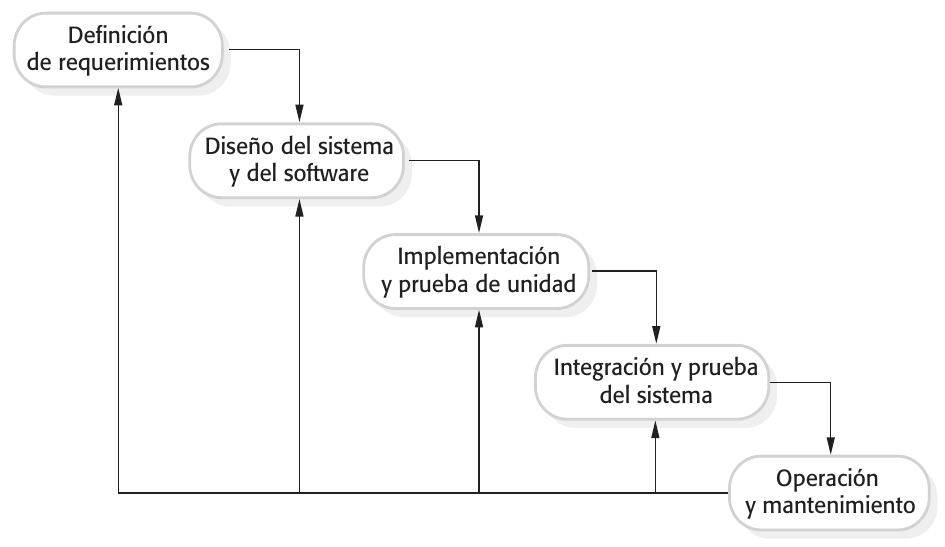
\includegraphics[width=0.9\textwidth]{imagenes/figura2_1.png} % Inserta una imagen
			
			\begin{flushleft}
				\hspace{1.20cm} \textbf{Nota.} Obtenido de \textcite{sommerville2011introduccion}. % Nota al pie para esta figura
			\end{flushleft}
			\vspace{-16pt}
			\label{fig:figura2_1} % Etiqueta para referencia cruzada
		\end{figure}
		
		
	\subsection{Análisis y definición de requerimientos}
		En esta fase inicial, se establecen los servicios, restricciones y objetivos del sistema en consulta con los usuarios. Todos estos elementos se definen en detalle y sirven como especificación del sistema \parencite{sommerville2011introduccion}.
		
		Esta fase implicaría identificar las necesidades de la empresa de transporte, como la gestión de la venta de boletos, el registro de encomiendas y la asignación de rutas de buses. Se debe trabajar con los principales interesados, como administradores y empleados de la empresa, para definir claramente los procesos actuales y los problemas que el software debería resolver.
	\subsection{Diseño del sistema y del software}
		El proceso de diseño del sistema divide los requerimientos en sistemas hardware o software. Establece una arquitectura completa del sistema. El diseño del software implica identificar y describir las abstracciones fundamentales del sistema software y sus relaciones \parencite{sommerville2011introduccion}.
		
		Esta fase incluiría el diseño de la arquitectura del sistema, la estructura de la base de datos y las interfaces de usuario para la gestión de buses y encomiendas.
	\subsection{Implementación y prueba de unidad}
		Durante esta etapa, el diseño del software se lleva a cabo como un conjunto o unidades de programas. La prueba de unidades implica verificar que cada una cumpla con su especificación \parencite{sommerville2011introduccion}.
		
		En esta etapa, se llevaría a cabo la programación del software utilizando herramientas adecuadas como lenguajes de programación, así como frameworks que permitan la integración de las funcionalidades necesarias para la venta de boletos, la gestión de encomiendas y la asignación de buses. El sistema debe permitir a los usuarios realizar transacciones, mientras que el backend gestionaría la logística de las rutas y encomiendas.
	\subsection{Integración y prueba de sistema}
		Los programas o las unidades individuales de programas se integran y prueban como un sistema completo para asegurar que se cumplan los requerimientos del software \parencite{sommerville2011introduccion}.
		
		Durante esta fase, se realizarían pruebas funcionales para garantizar que los procesos de venta de boletos, la gestión de encomiendas y la asignación de buses operen correctamente. Las pruebas incluirían la simulación de transacciones, el seguimiento de encomiendas y la verificación de la correcta asignación de rutas y conductores.
	\subsection{Operación y mantenimiento}
		Normalmente, esta es la fase más larga del ciclo de vida. El sistema se instala y se pone en uso práctico. El mantenimiento implica corregir errores no descubiertos en las etapas anteriores del ciclo de vida, mejorar la implementación de las unidades del sistema y resaltar los servicios del sistema una vez que se descubren nuevos requerimientos \parencite{sommerville2011introduccion}.
	\section{INGENIERÍA DE REQUERIMIENTOS}
		
		Algunas definiciones de la ingeniería de requerimientos son:
		
		Según \textcite{pressman2010ingenieria}, la ingeniería de requerimientos proporciona el mecanismo apropiado para entender lo que desea el cliente, analizar las necesidades, evaluar la factibilidad, negociar una solución razonable, especificar la solución sin ambigüedades, validar la especificación y administrar los requerimientos a medida que se transforman en un sistema funcional.
		
		De acuerdo a \textcite{sommerville2011introduccion}, la ingeniería de requerimientos establece la base para todas las fases posteriores del desarrollo de software, lo que la convierte en un proceso fundamental para garantizar el éxito del proyecto.
		
		Dadas las definiciones anteriores podemos decir que la ingeniería de requerimientos es: una parte importante del desarrollo de software porque se puede utilizar para definir y comprender las expectativas y necesidades de las personas que utilizan el sistema. Este proceso incluye diversas actividades enfocadas en la investigación, documentación, uso y gestión de requisitos de software para garantizar que el producto final satisfaga las necesidades del negocio y de los clientes, lo que también se clasifica en requerimientos funcionales y requerimientos no funcionales.
	\subsection{Requerimientos funcionales}
		Los requerimientos funcionales describen lo que el sistema debe hacer, es decir, las funciones o características específicas que se deben implementar. En este proyecto, los requerimientos funcionales incluirían aspectos como:
		\begin{itemize}[label=$\bullet$, left=0cm, labelsep = 1.05cm, topsep = 0pt, parsep = 0pt]
			\item Gestión de rutas y horarios
			\item Venta y reserva de boletos
			\item Asignación de asientos
			\item Registro y seguimiento de encomiendas
			\item Gestión de flota de buses
			\item Generación de reportes de ventas
			\item Manejo de perfiles de usuarios (administradores, empleados)
		\end{itemize}
	\subsection{Requerimientos no funcionales}
		Por otro lado, los requerimientos no funcionales especifican cómo debe funcionar el sistema en términos de rendimiento, usabilidad, seguridad y confiabilidad. Para el sistema, algunos de los requerimientos no funcionales incluyen:
		\begin{itemize}[label=$\bullet$, left=0cm, labelsep = 1.05cm, topsep = 0pt, parsep = 0pt]
			\item El sistema debe ser accesible desde múltiples dispositivos (computadoras, tablets y móviles).
			\item Garantizar la protección de los datos de los usuarios mediante protocolos de seguridad adecuados.
			\item Escalabilidad, capacidad de crecer para manejar aumento en usuarios y transacciones
			\item Mantenibilidad, arquitectura modular para facilitar actualizaciones
		\end{itemize}
	\subsection{Actividades de la ingeniería de requerimientos}
		Hay múltiples enfoques para definir las actividades de la ingeniería de requerimientos y la elección de un modelo particular a menudo depende del tamaño y la complejidad del software en desarrollo. Esto da lugar a la posibilidad de que se implementen diferentes actividades, las cuales pueden variar tanto en su cantidad como en su naturaleza.
		
		A continuación, se detallan las actividades que forman parte de la ingeniería de requerimientos para el presente proyecto:
		
		Paso 1: Levantamiento de requerimientos
		
		Paso 2: Análisis de requerimientos
		
		Paso 3: Especificación de requerimientos
		
		Paso 4: Validación de requerimientos
		
		Paso 5: Gestión de requerimientos\\
		\textbf{Paso 1: Levantamiento de requerimientos}
		
		En este primer paso se busca identificar, comprender y documentar las necesidades y expectativas de los usuarios y las partes interesadas respecto al sistema a desarrollar. Esta actividad es el primer paso en el ciclo de vida del software y se fundamenta en la interacción continua entre los desarrolladores, los usuarios y otros actores del proyecto. El objetivo principal es asegurar que el sistema refleje adecuadamente las funciones y características que se requieren, permitiendo que su implementación sea exitosa.
		
		La complejidad de esta fase radica en la diversidad de las fuentes de información y la posibilidad de que existan diferencias entre lo que los usuarios creen que necesitan y lo que realmente es necesario para el negocio. Según \textcite{sommerville2011introduccion}, uno de los mayores desafíos es interpretar correctamente las necesidades de los usuarios, ya que estos a menudo pueden tener una visión limitada del sistema o no ser conscientes de los detalles técnicos que implican sus solicitudes. Por ello, es fundamental contar con técnicas efectivas para recopilar esta información, como entrevistas, observación directa, cuestionarios y talleres participativos.
		
		Algunas de las técnicas más comunes y efectivas para el levantamiento de requerimientos son:
		
		Entrevistas: Son útiles para obtener información detallada y directa de los usuarios y otros interesados. Pueden ser estructuradas, semiestructuradas o no estructuradas, dependiendo de la profundidad de la información que se desee obtener. Las entrevistas permiten aclarar aspectos complejos y detectar necesidades particulares de cada usuario o área de la organización.
		
		De acuerdo a \textcite{diaz2013entrevista} en base a la clasificación antes mencionada se identifica que cada tipo de entrevista tiene su peculiaridad, sin embargo, en el momento de su desarrollo se presentan determinados momentos homogéneos. Estos momentos o fases de
		la entrevista los vemos en la figura \ref{fig:figura2_2}.
		
		\vspace{0.3cm} % Agregar 1 cm de espacio entre el párrafo y la figura
		
		\begin{figure}[h] % 'H' del paquete 'float' para mantener posición	
			\caption[Fases de la entrevista]
			{\newline Fases de la entrevista.} % Leyenda en la parte superior
			\vspace{0.3cm}
			\centering
			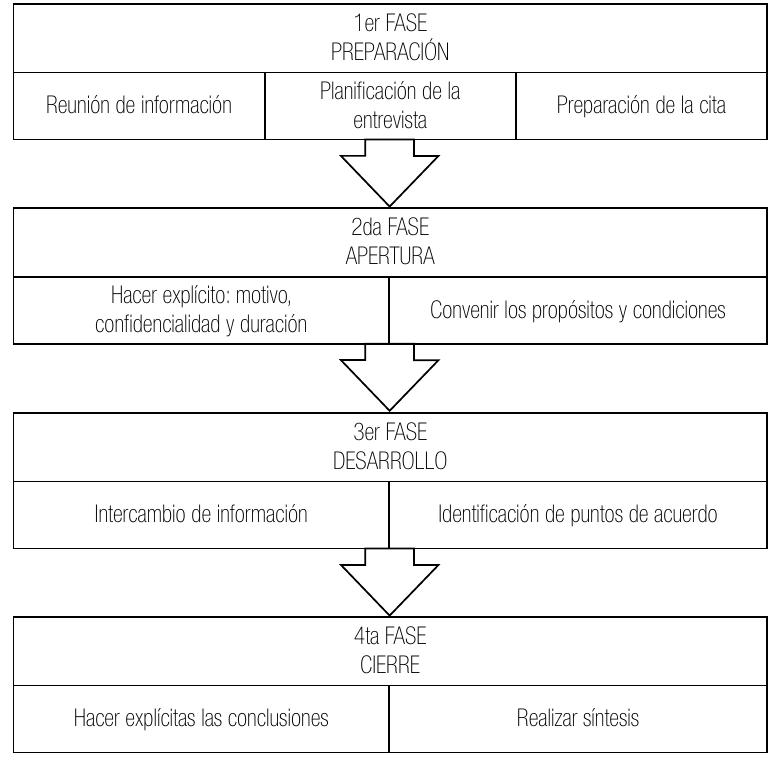
\includegraphics[width=0.65\textwidth]{imagenes/figura2_2.png} % Inserta una imagen
			\vspace{0.3cm}
			\caption*{\textup{\textbf{Nota}: Imagen tomada de \textcite{diaz2013entrevista}, \textit{La entrevista, recurso flexible.}}}
			\vspace{-0.8cm}
			\label{fig:figura2_2} % Etiqueta para referencia cruzada
		\end{figure}
		
		En conclusión \textcite{diaz2013entrevista} aclara que la entrevista es uno más de los instrumentos cuyo propósito es recabar datos, pero debido a su flexibilidad permite obtener información más profunda, detallada, que incluso el entrevistado y entrevistador no tenían identificada, ya que se adapta al contexto y a las características del entrevistado. Es valiosa en el campo de la investigación y más aún cuando se utiliza en estudios de tipo mixto como una visión complementaria del enfoque cuantitativo.
						
		Talleres de trabajo: Se utilizan para reunir a diferentes partes interesadas en un mismo espacio, facilitando la discusión colaborativa sobre los requerimientos. Estos talleres ayudan a resolver posibles conflictos entre usuarios y a consolidar una visión conjunta del sistema a desarrollar.
		
		Observación directa: Este enfoque implica observar a los usuarios en su entorno laboral para comprender mejor los procesos actuales, las dificultades que enfrentan y cómo un sistema nuevo podría mejorar su desempeño. La observación es particularmente útil cuando los usuarios no pueden articular claramente sus necesidades o cuando los problemas son inherentes a las tareas que realizan.
		
		Cuestionarios: Son una buena opción para obtener información de un amplio número de usuarios cuando no es posible realizar entrevistas individuales. Los cuestionarios permiten estructurar preguntas específicas sobre las necesidades del sistema, aunque son menos flexibles en cuanto a la obtención de respuestas detalladas.\\
		\textbf{Paso 2: Análisis de requerimientos}
		
		El análisis de requerimientos es donde se busca definir las necesidades y expectativas de los usuarios. Esta fase se enfoca en transformar las necesidades identificadas durante el levantamiento de requerimientos en especificaciones claras y comprensibles. Según \textcite{sommerville2011introduccion}, el análisis de requerimientos no solo implica la recopilación de datos, sino también su organización y priorización para asegurar que el producto final cumpla con las expectativas del cliente. Este proceso requiere un enfoque sistemático y la participación activa de todos los involucrados, lo que facilita la identificación de posibles problemas y la aclaración de dudas desde el inicio del proyecto.
		
		Durante el análisis de requerimientos, se documenta estos requerimientos, esto se realiza mediante el uso de herramientas de modelado, como diagramas de casos de uso, que permiten visualizar las interacciones entre los usuarios y el sistema. Además, el análisis ayuda a identificar requerimientos funcionales y no funcionales. La correcta identificación y documentación de estos requerimientos son fundamentales para evitar malosentendidos y garantizar que el desarrollo se alinee con las necesidades del cliente.
		
		El análisis también juega un papel esencial en la gestión del cambio, ya que a medida que se desarrolla el proyecto, pueden surgir nuevas necesidades o cambios en las prioridades del cliente. Por ello, es vital mantener una comunicación constante con las partes interesadas para ajustar los requerimientos de manera oportuna. A través de un análisis cuidadoso y dinámico, se pueden prevenir desviaciones en el proyecto y asegurar que el producto final se entregue dentro de los plazos y presupuestos establecidos.\\
		\textbf{Paso 3: Especificación de requerimientos}
		
		La especificación de requerimientos en el proceso de ingeniería de software, se trata de documentar y formalizar los requerimientos identificados durante la etapa de análisis. De acuerdo a \textcite{sommerville2011introduccion}, esta fase implica la creación de un documento que sirva como un contrato entre los desarrolladores y los interesados en el proyecto, asegurando que todas las partes tengan una comprensión clara de lo que se espera del sistema. La especificación debe ser clara, completa y comprensible, lo que facilita su uso como guía para el diseño, desarrollo y pruebas del software.
		
		Uno de los enfoques más utilizados en la especificación de requerimientos es el uso de historias de usuario, que permiten capturar las necesidades desde la perspectiva del usuario. Estas historias son breves descripciones que explican cómo un usuario interactuará con el sistema para lograr un objetivo específico. Según \textcite{cohn2004user}, este enfoque promueve una mejor comunicación entre los desarrolladores y los usuarios, ayuda a garantizar que se prioricen las características más valiosas del software. Además, las historias de usuario son fácilmente comprensibles, lo que las hace accesibles incluso para aquellos que no tienen un trasfondo técnico.
		
		Además de las historias de usuario, es común utilizar diagramas de casos de uso y modelos de datos para complementar la documentación de requerimientos. Los diagramas de casos de uso, como los propuestos por \textcite{booch2007object}, visualizan las interacciones entre los actores (usuarios o sistemas externos) y el sistema en desarrollo, ayudando a identificar las funcionalidades clave que deben implementarse. Por otro lado, los modelos de datos permiten definir la estructura de la información que el sistema gestionará, proporcionando una visión más profunda sobre cómo se relacionan los diferentes componentes de la aplicación.
		
		La especificación de requerimientos no es una actividad única; debe revisarse y actualizarse a medida que el proyecto avanza y se generan nuevos conocimientos. La inclusión de un proceso de revisión regular garantiza que los requerimientos sigan siendo relevantes y se adapten a cualquier cambio en las necesidades del negocio o en la tecnología disponible. Esta flexibilidad es esencial para el éxito del proyecto, ya que contribuye a la satisfacción del cliente y a la eficacia del equipo de desarrollo, minimizando el riesgo de retrabajo y asegurando una entrega más oportuna del producto final.\\
		\textbf{Paso 4: Validación de requerimientos}
		
		La validación de requerimientos es la etapa que tiene como objetivo asegurar que los requerimientos definidos son correctos, completos y viables antes de que el desarrollo del software continúe hacia etapas posteriores. \textcite{sommerville2011introduccion} subraya que la validación es el proceso mediante el cual se comprueba que los requerimientos son consistentes con las necesidades del cliente y cumplen con los objetivos del sistema.
		
		Entre las principales técnicas empleadas en la validación se encuentran las revisiones de los requerimientos, la construcción de prototipos, las simulaciones y el uso de casos de prueba. Estas actividades permiten identificar errores, inconsistencias o ambigüedades en la especificación, que podrían afectar la implementación del software. Según \textcite{pressman2010ingenieria}, uno de los principales riesgos en esta fase es la ambigüedad de los requerimientos, que podría resultar en un producto que no satisface las necesidades del cliente. Por tanto, se debe realizar revisiones exhaustivas y asegurar que todos los involucrados tengan una comprensión clara y compartida de lo que se debe desarrollar.
		
		La validación de requerimientos también busca garantizar que las funcionalidades propuestas sean técnicamente factibles y que el sistema final se ajuste a las restricciones legales y de seguridad. De acuerdo con \textcite{sommerville2011introduccion}, involucrar a los usuarios finales en el proceso de validación es vital, ya que son ellos quienes mejor pueden evaluar si los requerimientos reflejan sus necesidades reales. Esto puede lograrse mediante la creación de prototipos o modelos preliminares del sistema que permitan a los usuarios interactuar con el producto antes de su desarrollo completo.\\
		\textbf{Paso 5: Gestión de requerimientos}
		
		La gestión de requerimientos es una actividad que asegura que las necesidades, deseos y expectativas de las partes interesadas sean correctamente documentadas, monitoreadas y controladas a lo largo del ciclo de vida del proyecto. Esta tarea no finaliza una vez que los requerimientos han sido formalizados y especificados; en cambio, se extiende durante todo el desarrollo para asegurar que los cambios que surjan sean controlados adecuadamente, manteniendo la coherencia con los objetivos del proyecto.
		
		Una parte importante es el control de cambios, a lo largo del desarrollo de software, es común que los interesados soliciten modificaciones basadas en nuevas necesidades o la evolución del negocio. Aquí es donde la gestión de requerimientos entra en acción para evaluar, priorizar y aprobar o rechazar dichas modificaciones. Este proceso evita la introducción de cambios que puedan desestabilizar el proyecto, ayudando a prevenir sobrecostos o desviaciones del alcance.
		
		Otro aspecto importante es la trazabilidad de los requerimientos, que asegura que cada requerimiento pueda ser rastreado desde su origen, a través de su implementación y pruebas, hasta su entrega final. Por su parte \textcite{sommerville2011introduccion}, la trazabilidad facilita el seguimiento de cómo se cumplen los requerimientos durante las diferentes etapas del proyecto, lo que es esencial para garantizar que el software final cumpla con las expectativas originales de los interesados.
		
		Finalmente, la gestión de requerimientos también implica asegurar que la documentación de los requerimientos esté actualizada y disponible para todos. Mantener una buena comunicación y visibilidad sobre el estado de los requerimientos es fundamental para que los desarrolladores puedan alinearse con los objetivos del proyecto. Así, una correcta gestión de requerimientos contribuye a minimizar riesgos, optimizar recursos y garantizar el éxito del desarrollo del software.
				
	\section{MODELO ENTIDAD - RELACIÓN}
		El modelo entidad-relación (ER) es una herramienta fundamental en el diseño de bases de datos, que se utiliza para representar de manera gráfica la estructura de los datos y las relaciones entre ellos. Propuesto por Peter Chen en 1976, este modelo permite a los diseñadores de bases de datos conceptualizar y organizar la información de manera intuitiva, facilitando la comprensión de los requisitos del sistema antes de la implementación de la base de datos \parencite{theentity1976Chen}.
		
	\subsection{Componentes del modelo}
		
		\textbf{Entidades:} Se trata de cualquier objeto u elemento (real o abstracto) acerca del cual se pueda almacenar información en la base de datos. Es decir cualquier elemento informativo que tenga importancia para una base de datos y es representada por un rectángulo, dentro del cual se escribe lo que representa.
		
		\textbf{Relaciones:} Es una correspondencia o asociación entre dos o más entidades. Cada relación tiene un nombre que describe su función. Las relaciones se representan gráficamente mediante rombos y su nombre aparece en el interior.
		
		En el modelo entidad-relación, existen varios tipos de relaciones que describen cómo las entidades se conectan entre sí:
		
		Relación uno a uno (1:1): una entidad está relacionada exactamente con una instancia de otra entidad, y viceversa.
		
		Relación uno a muchos (1:N): una entidad está relacionada con varias instancias de otra entidad, pero una instancia de la segunda entidad está relacionada con solo una instancia de la primera entidad.
		
		Relación muchos a uno (N:1): muchas instancias de una entidad están relacionadas con una instancia de otra entidad.
		
		Relación muchos a muchos (N:N): muchas instancias de una entidad pueden estar relacionadas con muchas instancias de otra entidad, gestionada mediante una tabla de unión.
		
		\textbf{Atributos:} Estos son en esencia descripciones de las entidades o relaciones, que describen elementos y características básicos de éstas. Son fundamentales y establecen la información que deseamos almacenar de cada objeto de la base de datos.
		
		\textbf{Clave primaria:} Cada entidad tiene una clave primaria que la identifica de manera única dentro de la base de datos. La clave primaria es un atributo (o conjunto de atributos) que garantiza que no haya duplicados en la información.
		
		A continuación en la figura \ref{fig:figura2_3} podemos observar en ejemplo básico de un modelo entidad-relación.
		
		\vspace{0.3cm} % Agregar 1 cm de espacio entre el párrafo y la figura
		
		\begin{figure}[h] % 'H' del paquete 'float' para mantener posición	
			\caption[Ejemplo MER]
			{\newline Ejemplo de modelo entidad-relación.} % Leyenda en la parte superior
			\vspace{0.3cm}
			\centering
			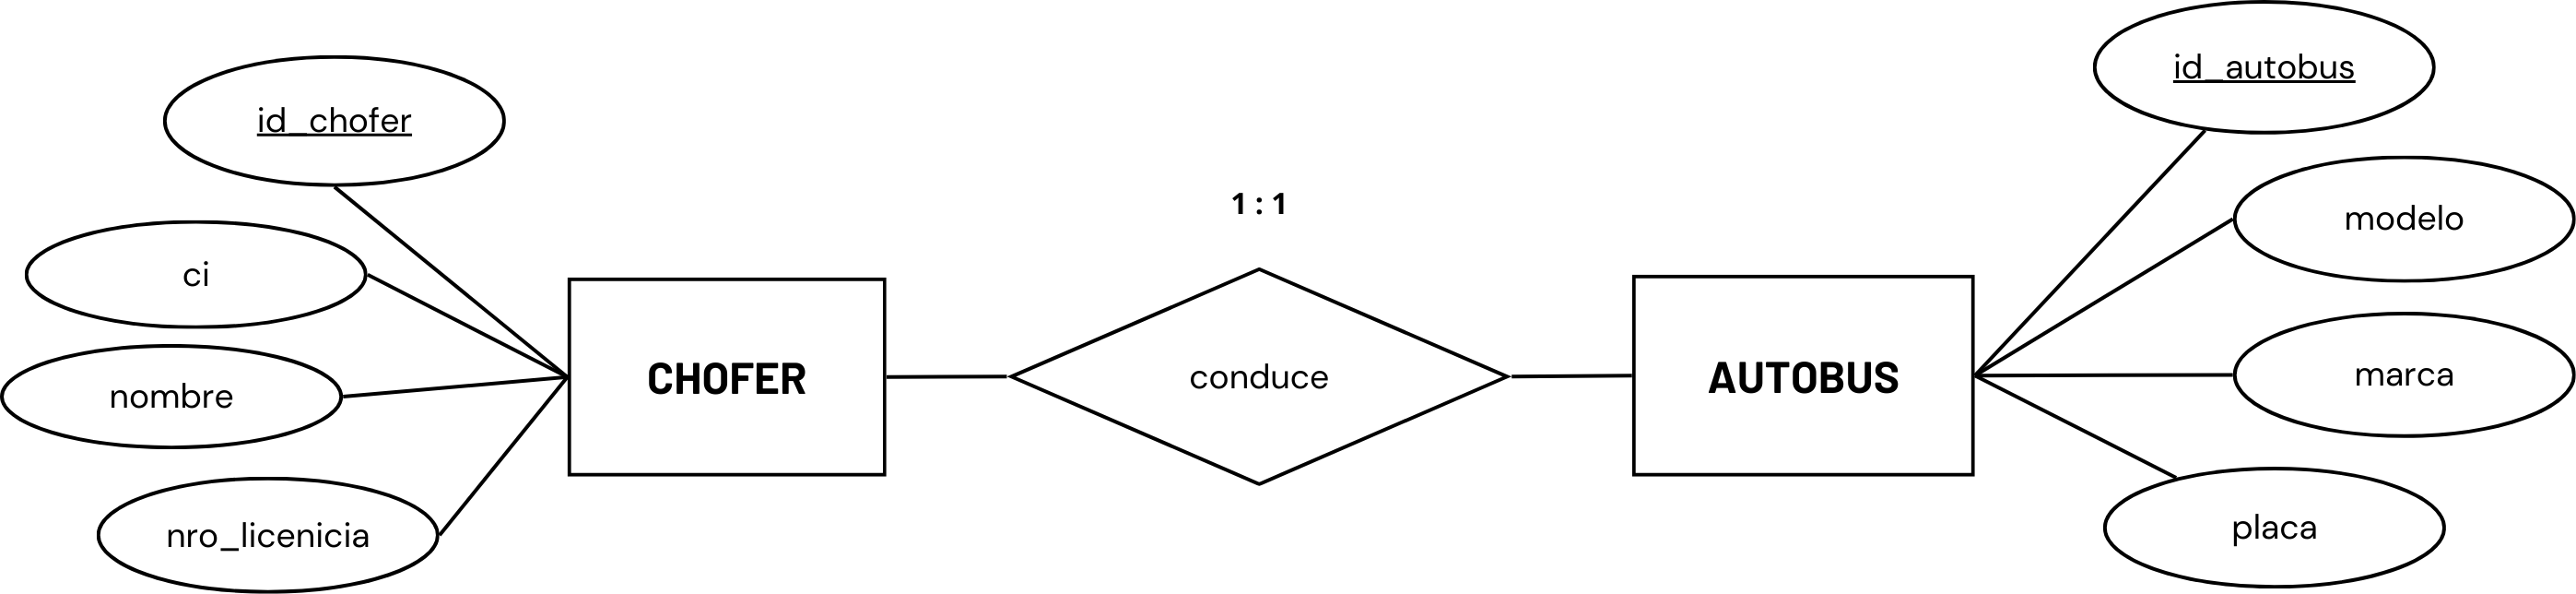
\includegraphics[width=0.9\textwidth]{imagenes/figura2_3.png} % Inserta una imagen
			\vspace{0.3cm}
			% \caption*{\textup{\textbf{Nota}: Obtenido de https://www.nngroup.com/}}
			\vspace{-0.6cm}
			\label{fig:figura2_3} % Etiqueta para referencia cruzada
		\end{figure}
	
	\section{BASE DE DATOS}
		La base de datos es un conjunto organizado de datos que se almacenan de manera estructurada y se gestionan a través de un sistema de gestión de bases de datos (SGBD). Su principal objetivo es facilitar el almacenamiento, recuperación y manipulación eficiente de grandes cantidades de información, asegurando la integridad y disponibilidad de los datos. La creación de una base de datos implica la definición de su estructura, basada en el modelo de datos elegido, que puede ser relacional, orientado a objetos, jerárquico, entre otros. El modelo relacional, propuesto por Edgar F. Codd en 1970, es el más utilizado hoy en día y organiza los datos en tablas compuestas por filas y columnas, conocidas como relaciones \parencite{codd1970relational}.
	\subsection{Base de datos relacional}
		Una base de datos relacional es un sistema de almacenamiento de información que organiza los datos en tablas interrelacionadas, conocidas como relaciones. Estas tablas están compuestas por filas (tuplas) y columnas (atributos), donde cada fila representa un registro único y cada columna un tipo de dato específico. Este modelo fue propuesto por Edgar F. Codd en 1970, en un esfuerzo por optimizar la gestión y manipulación de grandes cantidades de información, y se ha convertido en el enfoque predominante en la mayoría de las aplicaciones empresariales y científicas \textcite{codd1970relational}.
		
		Los Sistemas de Gestión de Bases de Datos Relacionales son software diseñado para gestionar bases de datos relacionales.
		
	\subsection{Modelo relacional}
		El modelo relacional, para el modelado y la gestión de bases de datos, es un modelo de datos basado en la lógica de predicados y en la teoría de conjuntos. Este modelo utiliza el lenguaje SQL (Structured Query Language) para realizar consultas, actualizar y gestionar los datos. Los componentes principales del modelo relacional son: Estructura de datos: Relaciones o tablas. Operadores: Conjunto de operaciones para manipular los datos (álgebra relacional). Restricciones de integridad: Reglas para mantener la consistencia de los datos.
		
	\subsection{Normalización}
		La normalización es el proceso de organización de una base de datos para reducir la redundancia y mejorar la integridad de los datos. Las formas normales más comunes son:
		
		Primera Forma Normal (1FN): Una tabla está en 1FN si todos sus atributos contienen valores atómicos (indivisibles) y cada entrada de la tabla tiene un único valor por columna. Es decir, no debe haber grupos repetidos ni atributos con listas de valores.
		
		Segunda Forma Normal (2FN): Para estar en 2FN, una tabla debe cumplir con la 1FN y, además, todos los atributos no clave deben depender completamente de la clave primaria. En otras palabras, elimina la dependencia parcial de los atributos en caso de que la clave primaria sea compuesta.
		
		Tercera Forma Normal (3FN): Una tabla está en 3FN si cumple con 2FN y no tiene dependencias transitivas. Esto significa que los atributos no clave no dependen de otros atributos no clave.
		
	\section{PATRÓN DE DISEÑO WEB}
		Los patrones de diseño web se refieren a un conjunto de principios que guían el desarrollo de páginas web y la creación de interfaces de usuario, abarcando desde elementos individuales hasta componentes más completos. A diferencia de las plantillas, que sirven como un punto de partida para diseñar páginas con una estructura similar pero con contenidos distintos, los patrones ofrecen un enfoque basado en buenas prácticas para el diseño. Utilizar estos patrones conlleva dos beneficios clave:
		
		Primero, aseguran una experiencia de usuario óptima al proporcionar directrices sobre la disposición y organización de los distintos elementos en una página, adaptándose así a las necesidades y expectativas de los usuarios.
		
		En segundo lugar, contribuyen a agilizar y simplificar el proceso de diseño, abordando problemas comunes en el desarrollo web que ya han encontrado soluciones efectivas.
		
	\section{DISEÑO EN FORMA DE F}
		
		El diseño en forma de "F" es un patrón de diseño web basado en el comportamiento natural de lectura de los usuarios, quienes escanean y consumen el contenido de las páginas web de una manera similar a la letra "F". Según \textcite{nielsen2006fshaped}, los usuarios tienden a leer primero horizontalmente, luego realizan una segunda mirada horizontal más corta y finalmente escanean hacia abajo de manera vertical, lo que crea la forma de la letra "F". Este comportamiento es clave para organizar el contenido en páginas de manera que optimice la visibilidad y la usabilidad como se puede ver en la figura \ref{fig:figura2_4}.
		
		\vspace{0.3cm} % Agregar 1 cm de espacio entre el párrafo y la figura
		
		\begin{figure}[h] % 'H' del paquete 'float' para mantener posición	
			\caption[Estudios de seguimiento ocular]
			{\newline Resultados de los estudios de seguimiento de los ojos.} % Leyenda en la parte superior
			\vspace{0.3cm}
			\centering
			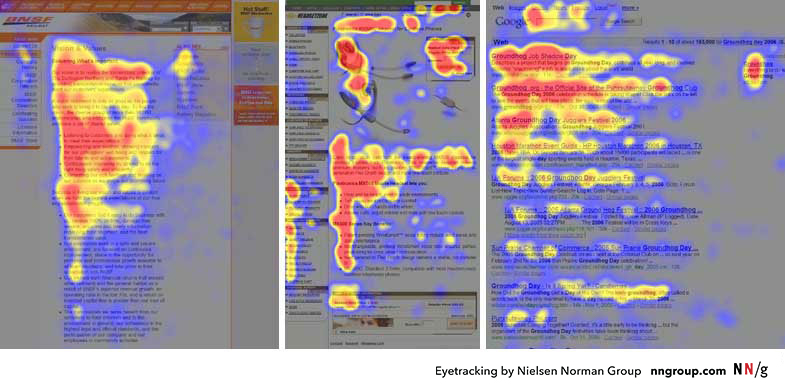
\includegraphics[width=0.85\textwidth]{imagenes/figura2_4.jpg} % Inserta una imagen
			\vspace{0.3cm}
			\caption*{\textup{\textbf{Nota}: Obtenido de https://www.nngroup.com/}}
			%\begin{flushleft}
			%	\hspace{1.20cm} \textit{Nota.} al pie asociada con esta figura, explicando detalles adicionales. % Nota al pie para esta figura
			%\end{flushleft}
			\vspace{-0.8cm}
			\label{fig:figura2_4} % Etiqueta para referencia cruzada
		\end{figure}
		
		En una web de administración, este modelo puede aplicarse eficazmente cuando se dispone un encabezado en la parte superior, un menú lateral izquierdo y el contenido principal en el centro:
		
		\textbf{Encabezado superior:} El encabezado se ubica en la parte superior de la página, el primer punto de atención visual de los usuarios, donde deberían colocarse elementos importantes como la identidad de la empresa, accesos a configuraciones o funciones críticas como el logout, ya que es la zona donde los usuarios enfocan su mirada inicialmente.
		
		\textbf{Menú lateral izquierdo:} El menú de navegación en el lado izquierdo está alineado con la columna vertical de la "F", lo que lo convierte en el lugar ideal para ubicar opciones de navegación. Las funciones más importantes deben estar en la parte superior del menú, donde los usuarios tienden a hacer un recorrido visual de arriba hacia abajo.
		
		\textbf{Contenido central:} El contenido principal de la página debería alinearse con las barras horizontales del patrón en forma de "F". La información más importante debe situarse en la parte superior, ya que esta área recibe más atención, mientras que las secciones menos cruciales pueden colocarse más abajo.
		
		\begin{figure}[h] % 'H' del paquete 'float' para mantener posición	
			\caption[Diseño en forma de F]
			{\newline Diseño en forma de F para la estructura de una web de administración.} % Leyenda en la parte superior
			\vspace{0.3cm}
			\centering
			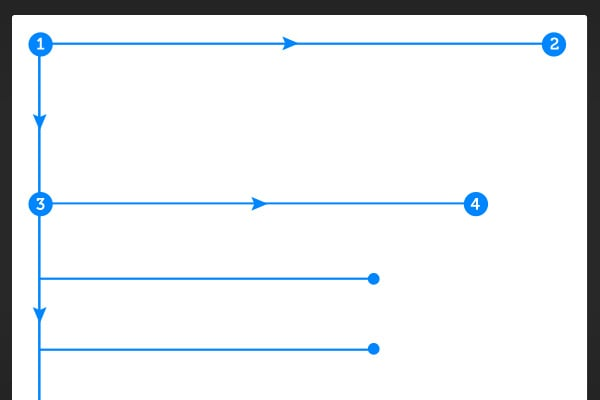
\includegraphics[width=0.75\textwidth]{imagenes/figura2_5.jpg} % Inserta una imagen
			\vspace{0.3cm}
			\caption*{\textup{\textbf{Nota}: Obtenido de https://webdesign.tutsplus.com/}}
			\vspace{-0.8cm}
			\label{fig:figura2_5} % Etiqueta para referencia cruzada
		\end{figure}
		
		En la figura \ref{fig:figura2_5} se ve que este diseño mejora la experiencia del usuario al seguir su comportamiento visual natural, lo que resulta en una mayor usabilidad y eficiencia en tareas administrativas. Según Nielsen (2006), el diseño en forma de F asegura que las áreas más importantes reciban la mayor atención, facilitando la navegación y el acceso a la información esencial:
	
	\section{PATRÓN DE ARQUITECTURA}
		Los patrones de arquitectura son soluciones generales y reutilizables para problemas comunes en el diseño de software. Estos patrones proporcionan un conjunto de subsistemas predefinidos, especifican sus responsabilidades e incluyen reglas y pautas para organizar las relaciones entre ellos. De acuerdo a \textcite{cervantes2016arquitectura}, los patrones de arquitectura se caracterizan por su capacidad de reutilización, abstracción, escalabilidad y mantenibilidad, lo que los convierte en herramientas fundamentales para el diseño de sistemas de software robustos y flexibles.
		
		La importancia de los patrones de arquitectura radica en su capacidad para representar la estructura fundamental de un sistema. Como señala \textcite{pressman2010ingenieria}, estos patrones "proporcionan un conjunto de subsistemas predefinidos, especifican sus responsabilidades e incluyen reglas y guías para organizar las relaciones entre los subsistemas". Estos patrones ofrecen un marco que guía la organización del código y la estructura de la aplicación, promoviendo la reutilización y facilitando el mantenimiento y la escalabilidad.
		
		La elección de un patrón de arquitectura adecuado influye en la calidad del software, su rendimiento y su facilidad de uso, el uso de patrones de arquitectura ayuda a los desarrolladores a afrontar la complejidad del software mediante la identificación de soluciones probadas y confiables, lo que contribuye a un desarrollo más ágil y eficiente. Este enfoque permite que los equipos de desarrollo colaboren de manera más efectiva, al tener una base común sobre la cual construir.
		
		Un patrón particularmente relevante en el desarrollo web es el Modelo-Vista-Controlador (MVC). Este patrón separa la lógica de negocio, la presentación y el control, permitiendo una mayor modularidad y flexibilidad en el diseño de aplicaciones web. 
		
	\section{PATRÓN MODELO-TEMPLATE-VIEW (MTV)}
		
		A partir del patrón MVC, han surgido variaciones adaptadas a las necesidades específicas de diferentes frameworks y lenguajes de programación. Una de estas variaciones es el patrón Modelo-Template-View (MTV), es un framework de desarrollo web de código abierto escrito en Python.
		
		El patrón MTV tiene la particularidad de separar claramente la lógica de la aplicación en tres componentes principales:
		
		\begin{itemize}[label=$\bullet$, left=0cm, labelsep = 1.05cm, topsep = 0pt, parsep = 0pt]
			\item \textbf{Model (Modelo)}: se refiere a la estructura de datos en Django, se define esta estructura creando una clase por cada tabla en la base de datos. Cada modelo de Django contiene los campos y comportamientos de los datos que desea almacenar.
			\item \textbf{Template (Plantilla)}: Es responsable de la presentación de los datos. Los templates permiten generar las vistas que el usuario final verá en la interfaz de la aplicación.
			\item \textbf{View (Vista)}: Actúa como intermediario entre el modelo y los templates, gestionando la lógica de la aplicación y determinando qué datos deben ser enviados a los templates.
		\end{itemize}
		
		La aplicación del patrón MTV en Django facilita la separación de responsabilidades, mejorando la mantenibilidad y la escalabilidad del sistema. Esta separación también permite que diferentes equipos puedan trabajar de manera independiente sobre cada componente, favoreciendo una mayor eficiencia en el desarrollo.		
	
	\section{HERRAMIENTAS DE DESARROLLO}
		En la tabla \ref{tab:tabla2_1}, tabla \ref{tab:tabla2_2} y tabla \ref{tab:tabla2_3} se identifican las herramientas de desarrollo que se utilizan para el proyecto.
		
		\begin{longtable}{>{\centering\arraybackslash}m{3cm} >{\centering\arraybackslash}m{5cm} >{\centering\arraybackslash}m{3cm}}
			\caption[Herramientas front-end]{\newline Herramientas a utilizar en el desarrollo del front-end del proyecto} \label{tab:tabla2_1}\\
			\toprule
			\textbf{Logo} & \textbf{Herramienta} & \textbf{Versión}\\
			\midrule
			\endfirsthead
			
			\toprule
			\textbf{Logo} & \textbf{Herramienta} & \textbf{Versión}\\
			\midrule
			\endhead
			
			\midrule
			\multicolumn{3}{r}{\textit{Continúa en la siguiente página}} \\
			\midrule
			\endfoot
			
			\bottomrule
			\endlastfoot
			
			% Aquí se colocan las filas de la tabla, por ejemplo:
			
\includegraphics[width=0.05\textwidth]{imagenes/logos/html.png}       & HTML & 5 \\
			
\includegraphics[width=0.05\textwidth]{imagenes/logos/css.png}       & CSS & 3 \\
			
\includegraphics[width=0.08\textwidth]{imagenes/logos/javascript.png}       & JavaScript & 6 \\
			
\includegraphics[width=0.09\textwidth]{imagenes/logos/bootstrap.png}       & Framework Bootstrap & 4 \\
			
		\end{longtable}
		\vspace{-12pt}  % O el valor que necesites para ajustar
		% Nota personalizada fuera de `\caption*{}`
		% \textbf{Nota}: Esta es la nota de la tabla, explicando datos relevantes.
					
		\begin{longtable}{>{\centering\arraybackslash}m{3cm} >{\centering\arraybackslash}m{5cm} >{\centering\arraybackslash}m{3cm}}
			\caption[Herramientas back-end]{\newline Herramientas a utilizar en el desarrollo del back-end del proyecto} \label{tab:tabla2_2}\\
			\toprule
			\textbf{Logo} & \textbf{Herramienta} & \textbf{Versión}\\
			\midrule
			\endfirsthead
			
			\toprule
			\textbf{Logo} & \textbf{Herramienta} & \textbf{Versión}\\
			\midrule
			\endhead
			
			\midrule
			\multicolumn{3}{r}{\textit{Continúa en la siguiente página}} \\
			\midrule
			\endfoot
			
			\bottomrule
			\endlastfoot
			
			% Aquí se colocan las filas de la tabla, por ejemplo:
			
\includegraphics[width=0.07\textwidth]{imagenes/logos/python.png}       & Python & 3.12.5 \\
			
\includegraphics[width=0.13\textwidth]{imagenes/logos/django.png}       & Framework Django & 5.11 \\
			
\includegraphics[width=0.08\textwidth]{imagenes/logos/postgre.png}       & PostgreSQL & 16.3 \\
			
\includegraphics[width=0.15\textwidth]{imagenes/logos/pgadmin.png}       & pgAdmin & 4 \\
			
		\end{longtable}
		\vspace{-12pt}  % O el valor que necesites para ajustar
		% Nota personalizada fuera de `\caption*{}`
		% \textbf{Nota}: Esta es la nota de la tabla, explicando datos relevantes.
				
		\begin{longtable}{>{\centering\arraybackslash}m{3cm} >{\centering\arraybackslash}m{5cm} >{\centering\arraybackslash}m{3cm}}
			\caption[Herramientas de programación]{\newline Herramientas a utilizar en programación y el control de versiones del proyecto} \label{tab:tabla2_3}\\
			\toprule
			\textbf{Logo} & \textbf{Herramienta} & \textbf{Versión}\\
			\midrule
			\endfirsthead
			
			\toprule
			\textbf{Logo} & \textbf{Herramienta} & \textbf{Versión}\\
			\midrule
			\endhead
			
			\midrule
			\multicolumn{3}{r}{\textit{Continúa en la siguiente página}} \\
			\midrule
			\endfoot
			
			\bottomrule
			\endlastfoot
			
			% Aquí se colocan las filas de la tabla, por ejemplo:
			
\includegraphics[width=0.1\textwidth]{imagenes/logos/vscode.png}       & Visual Studio Code & 1.94.2 \\
			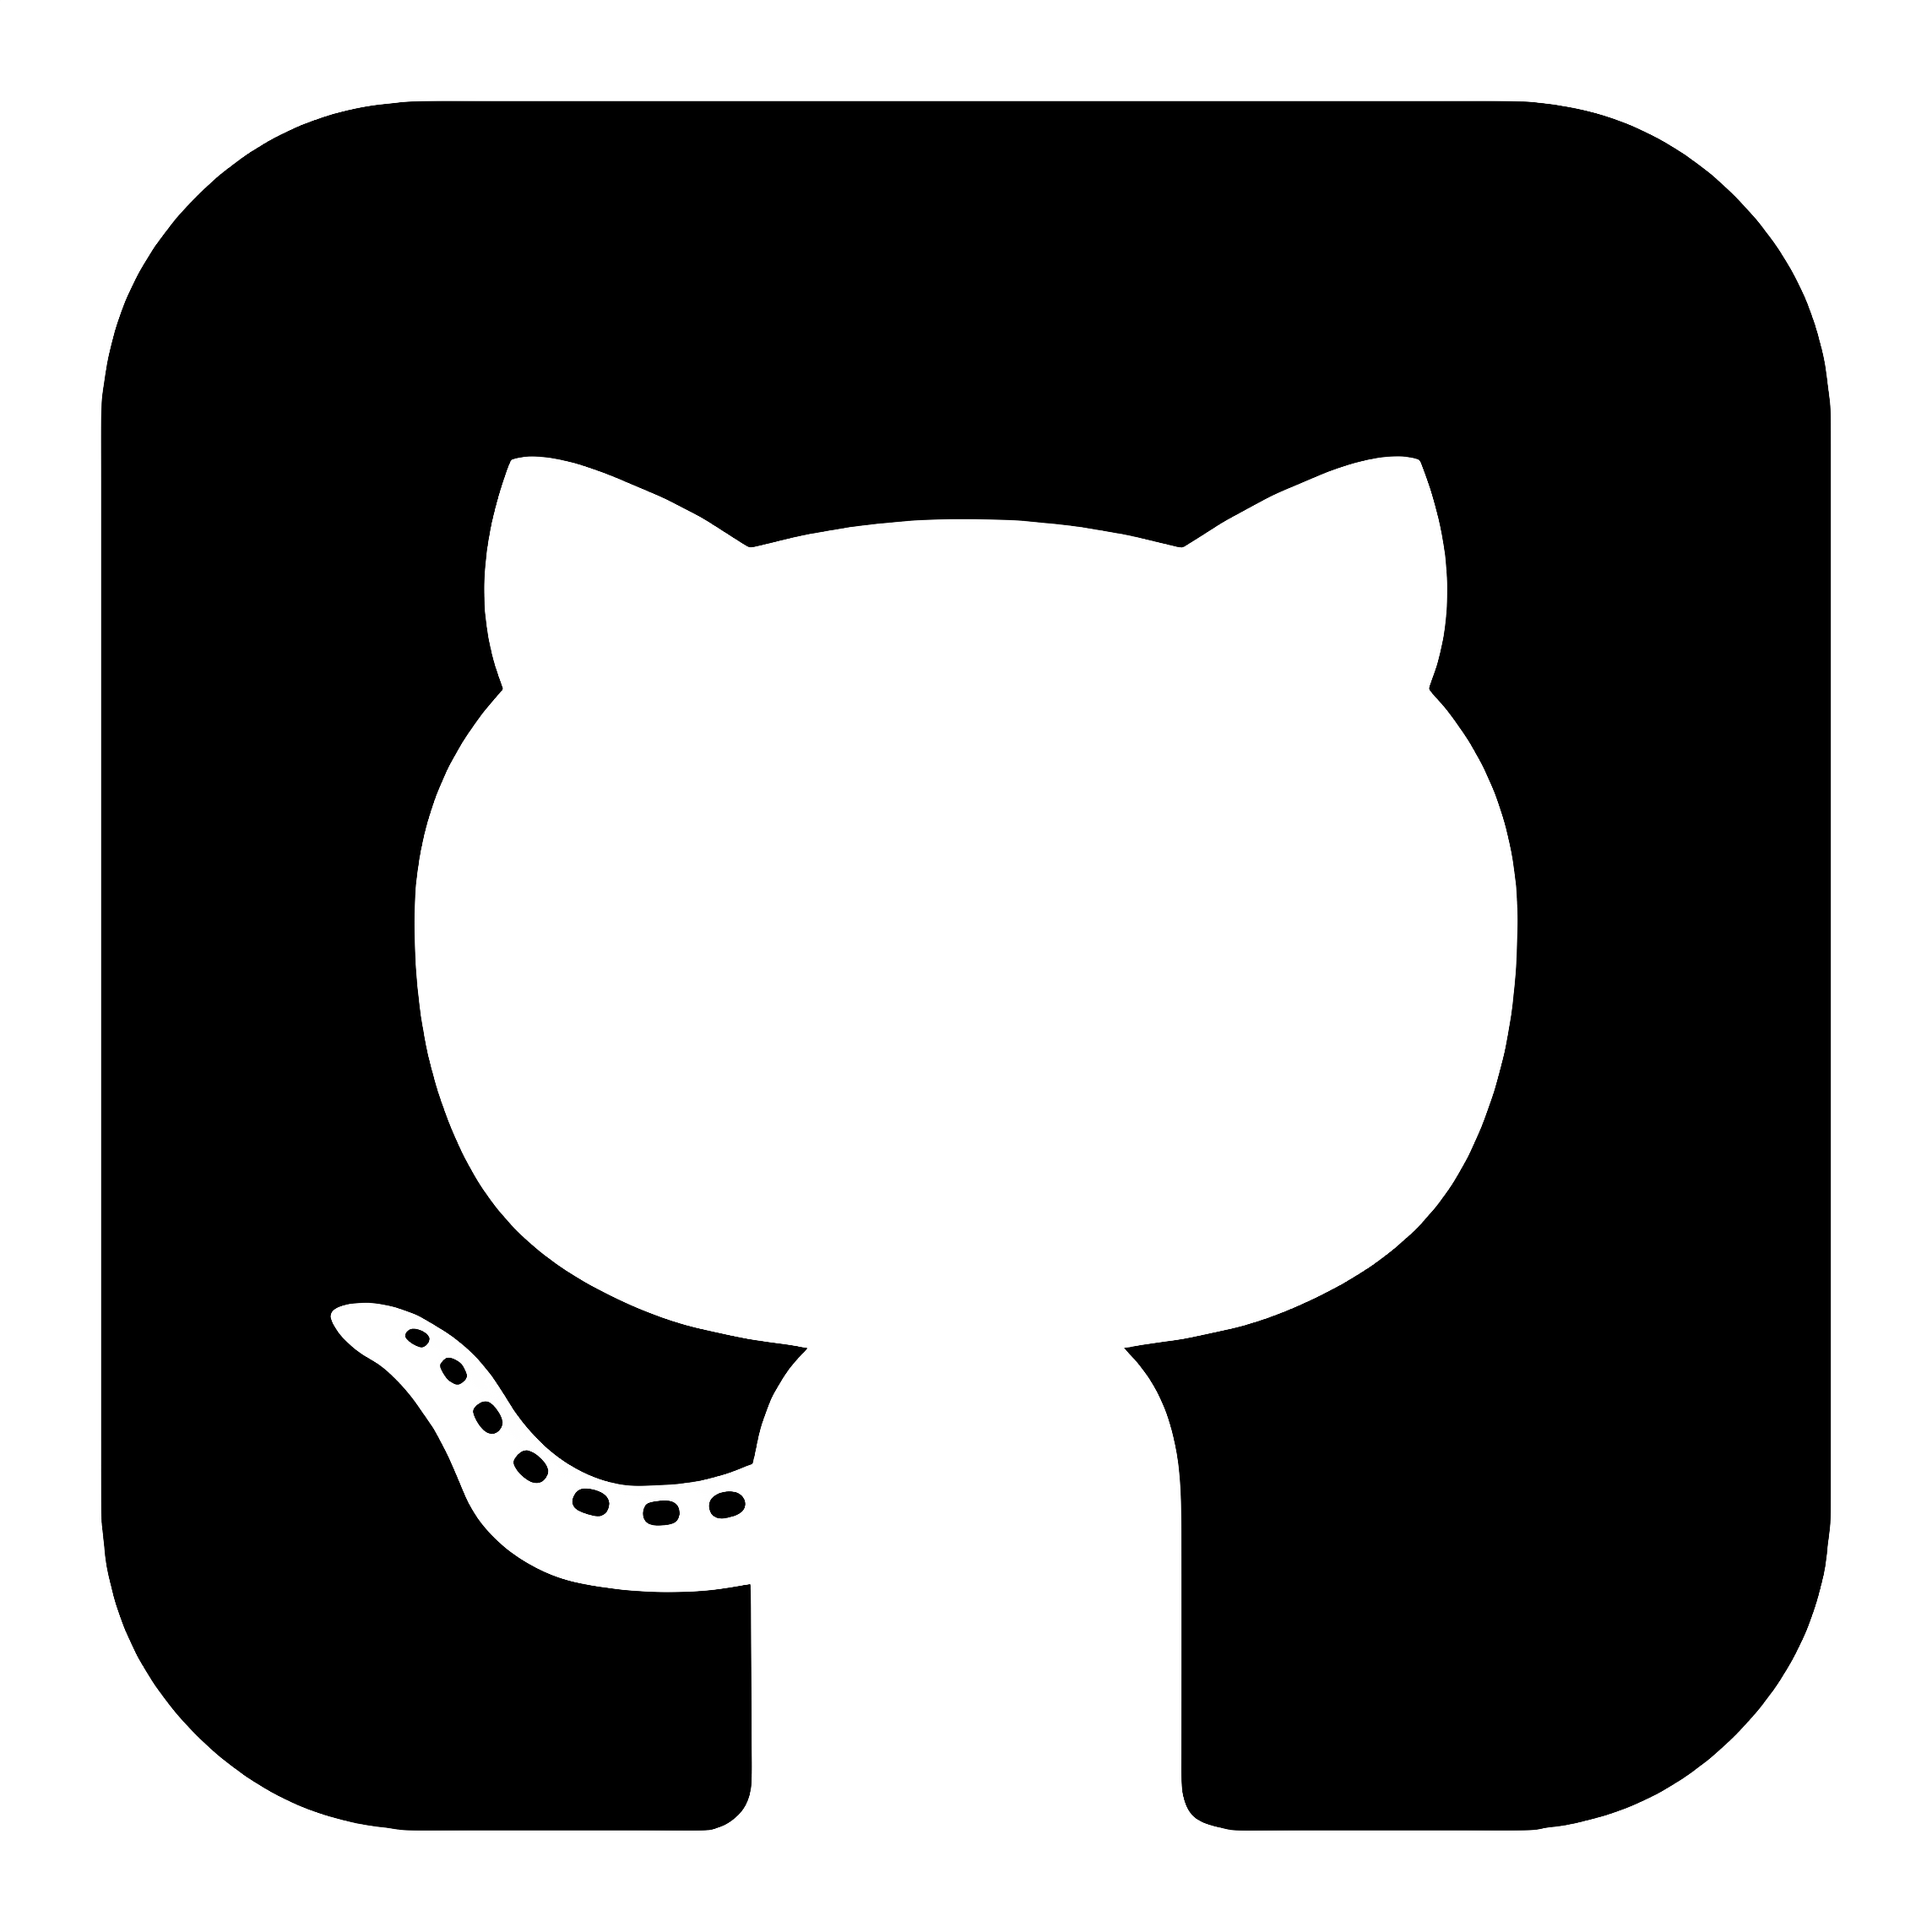
\includegraphics[width=0.07\textwidth]{imagenes/logos/github.png}       & Github & 2.46.1 \\	
			
		\end{longtable}
		\vspace{-12pt}  % O el valor que necesites para ajustar
		% Nota personalizada fuera de `\caption*{}`
		% \textbf{Nota}: Esta es la nota de la tabla, explicando datos relevantes.
		
	\section{PRUEBAS}
	\section{MODELO DE CALIDAD BOEHM}
		
	
	

	
	
	%\vspace{0.3cm} % Agregar 1 cm de espacio entre el párrafo y la figura
	
	%	\begin{figure}[h] % 'H' del paquete 'float' para mantener posición	
		%		\caption[Descripción corta]
		%		{\newline Resultados del informe PISA 2022.} % Leyenda en la parte superior
		%		\centering
		%		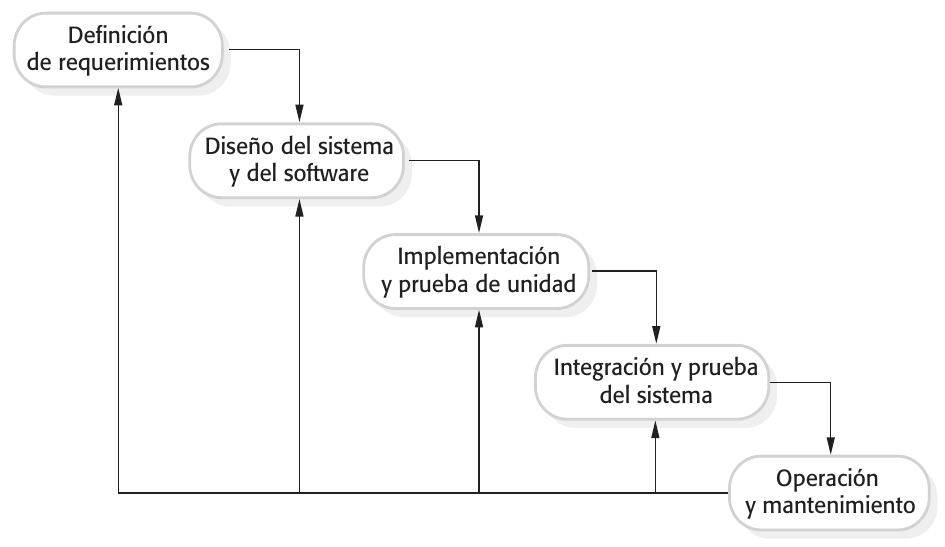
\includegraphics[width=0.95\textwidth]{imagenes/figura2_1.png} % Inserta una imagen
		%		
		%		\begin{flushleft}
			%			\hspace{1.20cm} \textit{Nota.} al pie asociada con esta figura, explicando detalles adicionales. % Nota al pie para esta figura
			%		\end{flushleft}
		%		\vspace{-16pt}
		%		\label{fig:figura2_1} % Etiqueta para referencia cruzada
		%	\end{figure}
	
	%\begin{table}[ht]
	%	\vspace{0.25cm}
	%	\centering
	%	\setstretch{2.0} % Establecer el espaciado a doble
		% \captionsetup{skip=0pt} % Sin espacio entre la tabla y el título
	%	\caption{\newline Herramientas a utilizar en el desarrollo del frontend del proyecto} \label{tab:tabla2_1}  % Título de la tabla
	%	\vspace{0.3cm}
		% \vspace{-\baselineskip} % Eliminar espacio arriba de la tabla
	%	\begin{tabular}{>{\centering\arraybackslash}m{3cm}>{\centering\arraybackslash}m{5cm}>{\centering\arraybackslash}m{3cm}}
			% \begin{tabular}{ccc} % Usar @{} para eliminar el espacio alrededor
				
	%			\toprule
	%			\textbf{Logo} & \textbf{Herramienta} & \textbf{Versión}\\
	%			\midrule
	%			
\includegraphics[width=0.05\textwidth]{imagenes/logos/html.png}       & HTML & 5 \\
	%			
\includegraphics[width=0.05\textwidth]{imagenes/logos/css.png}       & CSS & 3 \\
	%			
\includegraphics[width=0.08\textwidth]{imagenes/logos/javascript.png}       & JavaScript & 6 \\
	%			
\includegraphics[width=0.09\textwidth]{imagenes/logos/bootstrap.png}       & Framework Bootstrap & 4 \\
	%			\bottomrule
				
	%		\end{tabular}
	%		\vspace{0.7cm}
			% \vspace{-\baselineskip} % Eliminar espacio debajo de la tabla
			% \caption*{\textup{\textbf{Nota}: Esta es la nota de la tabla, explicando datos relevantes.}}
	%		\vspace{-1cm} % Eliminar espacio debajo de la tabla
	%	\end{table}


